%%%%%%%%%%%%%%%%%%%%%%%%%%%%%%%%%%%%%%%%
% datoteka diploma-FRI-vzorec.tex
%
%POZOR: ta verzija ne producira pdf datoteke v pdf/A formatu!!!
%namenjena je le za nalogo pri Diplomskem seminarju!
%
% vzorčna datoteka za pisanje diplomskega dela v formatu LaTeX
% na UL Fakulteti za računalništvo in informatiko
%
% na osnovi starejših verzij vkup spravil Franc Solina, maj 2021
% prvo verzijo je leta 2010 pripravil Gašper Fijavž
%
% za upravljanje z literaturo ta vezija uporablja BibLaTeX
%
% svetujemo uporabo Overleaf.com - na tej spletni implementaciji LaTeXa ta vzorec zagotovo pravilno deluje
%

\documentclass[a4paper,12pt,openright]{book}
%\documentclass[a4paper, 12pt, openright, draft]{book}  Nalogo preverite tudi z opcijo draft, ki pokaže, katere vrstice so predolge! Pozor, v draft opciji, se slike ne pokažejo!

\usepackage[utf8]{inputenc}   % omogoča uporabo slovenskih črk kodiranih v formatu UTF-8
\usepackage[slovene,english]{babel}    % naloži, med drugim, slovenske delilne vzorce
\usepackage[pdftex]{graphicx}  % omogoča vlaganje slik različnih formatov
\usepackage{fancyhdr}          % poskrbi, na primer, za glave strani
\usepackage{amssymb}           % dodatni matematični simboli
\usepackage{amsmath}           % eqref, npr.
\usepackage{hyperxmp}
\usepackage[hyphens]{url}
\usepackage{csquotes}
\usepackage[pdftex, colorlinks=true,
    citecolor=black, filecolor=black,
    linkcolor=black, urlcolor=black,
    pdfproducer={LaTeX}, pdfcreator={LaTeX}]{hyperref}

\usepackage{color}
\usepackage{soul}

\usepackage[
    backend=biber,
    style=numeric,
    sorting=nty,
]{biblatex}


\addbibresource{literatura.bib} %Imports bibliography file


%%%%%%%%%%%%%%%%%%%%%%%%%%%%%%%%%%%%%%%%
%	DIPLOMA INFO
%%%%%%%%%%%%%%%%%%%%%%%%%%%%%%%%%%%%%%%%
\newcommand{\ttitle}{Nevroevolucija za strojno učenje}
\newcommand{\ttitleEn}{Neuroevolution for machine learning}
\newcommand{\tsubject}{\ttitle}
\newcommand{\tsubjectEn}{\ttitleEn}
\newcommand{\tauthor}{Jure Vreček}
\newcommand{\tkeywords}{nevroevolucija, strojno učenje, nevronske mreže}
\newcommand{\tkeywordsEn}{neuroevolution, machine learning, neural nets}

%%%%%%%%%%%%%%%%%%%%%%%%%%%%%%%%%%%%%%%%
%	HYPERREF SETUP
%%%%%%%%%%%%%%%%%%%%%%%%%%%%%%%%%%%%%%%%
\hypersetup{pdftitle={\ttitle}}
\hypersetup{pdfsubject=\ttitleEn}
\hypersetup{pdfauthor={\tauthor}}
\hypersetup{pdfkeywords=\tkeywordsEn}

%%%%%%%%%%%%%%%%%%%%%%%%%%%%%%%%%%%%%%%%
% postavitev strani
%%%%%%%%%%%%%%%%%%%%%%%%%%%%%%%%%%%%%%%%

\addtolength{\marginparwidth}{-20pt} % robovi za tisk
\addtolength{\oddsidemargin}{40pt}
\addtolength{\evensidemargin}{-40pt}

\renewcommand{\baselinestretch}{1.3} % ustrezen razmik med vrsticami
\setlength{\headheight}{15pt}        % potreben prostor na vrhu
\renewcommand{\chaptermark}[1]%
{\markboth{\MakeUppercase{\thechapter.\ #1}}{}} \renewcommand{\sectionmark}[1]%
{\markright{\MakeUppercase{\thesection.\ #1}}} \renewcommand{\headrulewidth}{0.5pt} \renewcommand{\footrulewidth}{0pt}
\fancyhf{}
\fancyhead[LE,RO]{\sl \thepage}
%\fancyhead[LO]{\sl \rightmark} \fancyhead[RE]{\sl \leftmark}
\fancyhead[RE]{\sc \tauthor}              % dodal Solina
\fancyhead[LO]{\sc Diplomska naloga}     % dodal Solina


\newcommand{\BibLaTeX}{{\sc Bib}\LaTeX}
\newcommand{\BibTeX}{{\sc Bib}\TeX}

%%%%%%%%%%%%%%%%%%%%%%%%%%%%%%%%%%%%%%%%
% naslovi
%%%%%%%%%%%%%%%%%%%%%%%%%%%%%%%%%%%%%%%%

\newcommand{\autfont}{\Large}
\newcommand{\titfont}{\LARGE\bf}
\newcommand{\clearemptydoublepage}{\newpage{\pagestyle{empty}\cleardoublepage}}
\setcounter{tocdepth}{1}          % globina kazala

%%%%%%%%%%%%%%%%%%%%%%%%%%%%%%%%%%%%%%%%
% konstrukti
%%%%%%%%%%%%%%%%%%%%%%%%%%%%%%%%%%%%%%%%
\newtheorem{izrek}{Izrek}[chapter]
\newtheorem{trditev}{Trditev}[izrek]
\newenvironment{dokaz}{\emph{Dokaz.}\ }{\hspace{\fill}{$\Box$}}


%%%%%%%%%%%%%%%%%%%%%%%%%%%%%%%%%%%%%%%%%%%%%%%%%%%%%%%%%%%%%%%%%%%%%%%%%%%%%%%
%% PDF-A
%%%%%%%%%%%%%%%%%%%%%%%%%%%%%%%%%%%%%%%%%%%%%%%%%%%%%%%%%%%%%%%%%%%%%%%%%%%%%%%

%%%%%%%%%%%%%%%%%%%%%%%%%%%%%%%%%%%%%%%%
% define medatata
%%%%%%%%%%%%%%%%%%%%%%%%%%%%%%%%%%%%%%%%
\def\Title{\ttitle}
\def\Author{\tauthor, jv9074@fri.uni-lj.si}
\def\Subject{\ttitleEn}
\def\Keywords{\tkeywordsEn}

%%%%%%%%%%%%%%%%%%%%%%%%%%%%%%%%%%%%%%%%
% \convertDate converts D:20080419103507+02'00' to 2008-04-19T10:35:07+02:00
%%%%%%%%%%%%%%%%%%%%%%%%%%%%%%%%%%%%%%%%
\def\convertDate{%
    \getYear
}

{\catcode`\D=12
\gdef\getYear D:#1#2#3#4{\edef\xYear{#1#2#3#4}\getMonth}
}
\def\getMonth#1#2{\edef\xMonth{#1#2}\getDay}
\def\getDay#1#2{\edef\xDay{#1#2}\getHour}
\def\getHour#1#2{\edef\xHour{#1#2}\getMin}
\def\getMin#1#2{\edef\xMin{#1#2}\getSec}
\def\getSec#1#2{\edef\xSec{#1#2}\getTZh}
\def\getTZh +#1#2{\edef\xTZh{#1#2}\getTZm}
\def\getTZm '#1#2'{%
    \edef\xTZm{#1#2}%
    \edef\convDate{\xYear-\xMonth-\xDay T\xHour:\xMin:\xSec+\xTZh:\xTZm}%
}

%\expandafter\convertDate\pdfcreationdate

%%%%%%%%%%%%%%%%%%%%%%%%%%%%%%%%%%%%%%%%
% get pdftex version string
%%%%%%%%%%%%%%%%%%%%%%%%%%%%%%%%%%%%%%%%
\newcount\countA
\countA=\pdftexversion
\advance \countA by -100
\def\pdftexVersionStr{pdfTeX-1.\the\countA.\pdftexrevision}


%%%%%%%%%%%%%%%%%%%%%%%%%%%%%%%%%%%%%%%%
% XMP data
%%%%%%%%%%%%%%%%%%%%%%%%%%%%%%%%%%%%%%%%
\usepackage{xmpincl}
%\includexmp{pdfa-1b}

%%%%%%%%%%%%%%%%%%%%%%%%%%%%%%%%%%%%%%%%
% pdfInfo
%%%%%%%%%%%%%%%%%%%%%%%%%%%%%%%%%%%%%%%%
\pdfinfo{%
    /Title    (\ttitle)
    /Author   (\tauthor, damjan@cvetan.si)
    /Subject  (\ttitleEn)
    /Keywords (\tkeywordsEn)
    /ModDate  (\pdfcreationdate)
    /Trapped /False
}

%%%%%%%%%%%%%%%%%%%%%%%%%%%%%%%%%%%%%%%%
% znaki za copyright stran
%%%%%%%%%%%%%%%%%%%%%%%%%%%%%%%%%%%%%%%%

\newcommand{\CcImageCc}[1]{%
    
\includegraphics[scale=#1]{cc_cc_30}%
}
\newcommand{\CcImageBy}[1]{%
    
\includegraphics[scale=#1]{cc_by_30}%
}
\newcommand{\CcImageSa}[1]{%
    
\includegraphics[scale=#1]{cc_sa_30}%
}

%%%%%%%%%%%%%%%%%%%%%%%%%%%%%%%%%%%%%%%%%%%%%%%%%%%%%%%%%%%%%%%%%%%%%%%%%%%%%%%
%%%%%%%%%%%%%%%%%%%%%%%%%%%%%%%%%%%%%%%%%%%%%%%%%%%%%%%%%%%%%%%%%%%%%%%%%%%%%%%

\begin{document}
    \selectlanguage{slovene}
    \frontmatter
    \setcounter{page}{1} %
    \renewcommand{\thepage}{}       % preprečimo težave s številkami strani v kazalu

%%%%%%%%%%%%%%%%%%%%%%%%%%%%%%%%%%%%%%%%
%naslovnica
    \thispagestyle{empty}%
    \begin{center}
    {\large\sc Univerza v Ljubljani\\%
    Fakulteta za računalništvo in informatiko\\%
    }
        \vskip 10em%
            {\autfont \tauthor\par}%
            {\titfont \ttitle \par}%
            {\vskip 3em \textsc{DIPLOMSKO DELO\\[5mm]         % dodal Solina za ostale študijske programe
%    VISOKOŠOLSKI STROKOVNI ŠTUDIJSKI PROGRAM\\ PRVE STOPNJE\\ RAČUNALNIŠTVO IN INFORMATIKA}\par}%
        UNIVERZITETNI ŠTUDIJSKI PROGRAM\\ PRVE STOPNJE\\ RAČUNALNIŠTVO IN INFORMATIKA}\par}%
%    INTERDISCIPLINARNI UNIVERZITETNI\\ ŠTUDIJSKI PROGRAM PRVE STOPNJE\\ MULTIMEDIJA}\par}%
%    INTERDISCIPLINARNI UNIVERZITETNI\\ ŠTUDIJSKI PROGRAM PRVE STOPNJE\\ UPRAVNA INFORMATIKA}\par}%
%    INTERDISCIPLINARNI UNIVERZITETNI\\ ŠTUDIJSKI PROGRAM PRVE STOPNJE\\ RAČUNALNIŠTVO IN MATEMATIKA}\par}%
        \vfill\null%
% izberite pravi habilitacijski naziv mentorja!
        {\large \textsc{Mentor}: prof. dr. Marko Robnik Šikonja\par}%
%   {\large \textsc{Somentor}:  viš. pred./doc./izr. prof./prof. dr.  Martin Krpan \par}%
        {\vskip 2em \large Ljubljana, \the\year \par}%
    \end{center}
% prazna stran
%\clearemptydoublepage
% izjava o licencah itd. se izpiše na hrbtni strani naslovnice

%%%%%%%%%%%%%%%%%%%%%%%%%%%%%%%%%%%%%%%%
%copyright stran
%%%%%%%%%%%%%%%%%%%%%%%%%%%%%%%%%%%%%%%%
    \newpage
    \thispagestyle{empty}

    \vspace*{5cm}
    {\small \noindent
    To delo je ponujeno pod licenco \textit{Creative Commons Priznanje avtorstva-Deljenje pod enakimi pogoji 2.5 Slovenija} (ali novej\v so razli\v cico).
    To pomeni, da se tako besedilo, slike, grafi in druge sestavine dela kot tudi rezultati diplomskega dela lahko prosto distribuirajo,
        reproducirajo, uporabljajo, priobčujejo javnosti in predelujejo, pod pogojem, da se jasno in vidno navede avtorja in naslov tega
    dela in da se v primeru spremembe, preoblikovanja ali uporabe tega dela v svojem delu, lahko distribuira predelava le pod
    licenco, ki je enaka tej.
    Podrobnosti licence so dostopne na spletni strani \href{http://creativecommons.si}{creativecommons.si} ali na Inštitutu za
    intelektualno lastnino, Streliška 1, 1000 Ljubljana.

    \vspace*{1cm}
        \begin{center}% 0.66 / 0.89 = 0.741573033707865
            \CcImageCc{0.741573033707865}\hspace*{1ex}\CcImageBy{1}\hspace*{1ex}\CcImageSa{1}%
        \end{center}
    }

    \vspace*{1cm}
    {\small \noindent
    Izvorna koda diplomskega dela, njeni rezultati in v ta namen razvita programska oprema je ponujena pod licenco GNU General Public License,
        različica 3 (ali novejša). To pomeni, da se lahko prosto distribuira in/ali predeluje pod njenimi pogoji.
    Podrobnosti licence so dostopne na spletni strani \url{http://www.gnu.org/licenses/}.
    }

    \vfill
    \begin{center}
        \ \\ \vfill
        {\em
        Besedilo je oblikovano z urejevalnikom besedil \LaTeX.}
    \end{center}

% prazna stran
    \clearemptydoublepage

%%%%%%%%%%%%%%%%%%%%%%%%%%%%%%%%%%%%%%%%
% stran 3 med uvodnimi listi
    \thispagestyle{empty}
    \
    \vfill

    \bigskip
    \noindent\textbf{Kandidat:} Jure Vreček\\
    \noindent\textbf{Naslov:} Neuroevolucija za strojno učenje\\
% vstavite ustrezen naziv študijskega programa!
    \noindent\textbf{Vrsta naloge:} Diplomska naloga na univerzitetnem programu prve stopnje Računalništvo in informatika \\
% izberite pravi habilitacijski naziv mentorja!
    \noindent\textbf{Mentor:} prof. dr. Marko Robnik Šikonja\\
    %\noindent\textbf{Somentor:} isto kot za mentorja

    \bigskip
    \noindent\textbf{Opis:}\\
    Besedilo teme diplomskega dela študent prepiše iz študijskega informacijskega sistema, kamor ga je vnesel mentor.
    V nekaj stavkih bo opisal, kaj pričakuje od kandidatovega diplomskega dela.
    Kaj so cilji, kakšne metode naj uporabi, morda bo zapisal tudi ključno literaturo.

    \bigskip
    \noindent\textbf{Title:} Neuroevolution for machine learning

    \bigskip
    \noindent\textbf{Description:}\\
    opis diplome v angleščini

    \vfill



    \vspace{2cm}

% prazna stran
    \clearemptydoublepage

% zahvala
    \thispagestyle{empty}\mbox{}\vfill\null\it%
    \noindent
    Na tem mestu zapišite, komu se zahvaljujete za pomoč pri izdelavi diplomske naloge oziroma pri vašem študiju nasploh. Pazite, da ne boste koga pozabili. Utegnil vam bo zameriti. Temu se da izogniti tako, da celotno zahvalo izpustite.
    \rm\normalfont

% prazna stran
    \clearemptydoublepage

%%%%%%%%%%%%%%%%%%%%%%%%%%%%%%%%%%%%%%%%
% posvetilo, če sama zahvala ne zadošča :-)
    \thispagestyle{empty}\mbox{}{\vskip0.20\textheight}\mbox{}\hfill\begin{minipage}{0.55\textwidth}%
                                                                        Svoji dragi Alenčici.
                                                                        \normalfont
    \end{minipage}

% prazna stran
    \clearemptydoublepage


%%%%%%%%%%%%%%%%%%%%%%%%%%%%%%%%%%%%%%%%
% kazalo
    \pagestyle{empty}
    \def\thepage{}% preprečimo težave s številkami strani v kazalu
    \tableofcontents{}


% prazna stran
    \clearemptydoublepage

%%%%%%%%%%%%%%%%%%%%%%%%%%%%%%%%%%%%%%%%
% seznam kratic

    \chapter*{Seznam uporabljenih kratic}

    \noindent\begin{tabular}{p{0.11\textwidth}|p{.39\textwidth}|p{.39\textwidth}}    % po potrebi razširi prvo kolono tabele na račun drugih dveh!
    {\bf kratica}
                 & {\bf angleško}             & {\bf slovensko}                       \\ \hline
                 {\bf CA}   & classification accuracy    & klasifikacijska točnost \\
                 {\bf DBMS} & database management system & sistem za upravljanje podatkovnih baz \\
                 {\bf SVM}  & support vector machine     & metoda podpornih vektorjev            \\
%  \dots & \dots & \dots \\
    \end{tabular}


% prazna stran
    \clearemptydoublepage

%%%%%%%%%%%%%%%%%%%%%%%%%%%%%%%%%%%%%%%%
% povzetek
    \addcontentsline{toc}{chapter}{Povzetek}
    \chapter*{Povzetek}

    \noindent\textbf{Naslov:} \ttitle
    \bigskip

    \noindent\textbf{Avtor:} \tauthor
    \bigskip

%\noindent\textbf{Povzetek:}
    \noindent V vzorcu je predstavljen postopek priprave diplomskega dela z uporabo okolja \LaTeX. Vaš povzetek mora sicer vsebovati približno 100 besed, ta tukaj je odločno prekratek.
    Dober povzetek vključuje: (1) kratek opis obravnavanega problema, (2) kratek opis vašega pristopa za reševanje tega problema in (3) (najbolj uspešen) rezultat ali prispevek diplomske naloge.

    \bigskip

    \noindent\textbf{Ključne besede:} \tkeywords.
% prazna stran
    \clearemptydoublepage

%%%%%%%%%%%%%%%%%%%%%%%%%%%%%%%%%%%%%%%%
% abstract
    \selectlanguage{english}
    \addcontentsline{toc}{chapter}{Abstract}
    \chapter*{Abstract}

    \noindent\textbf{Title:} \ttitleEn
    \bigskip

    \noindent\textbf{Author:} \tauthor
    \bigskip

%\noindent\textbf{Abstract:}
    \noindent This sample document presents an approach to typesetting your BSc thesis using \LaTeX.
    A proper abstract should contain around 100 words which makes this one way too short.
    \bigskip

    \noindent\textbf{Keywords:} \tkeywordsEn.
    \selectlanguage{slovene}
% prazna stran
    \clearemptydoublepage

%%%%%%%%%%%%%%%%%%%%%%%%%%%%%%%%%%%%%%%%
    \mainmatter
    \setcounter{page}{1}
    \pagestyle{fancy}


    \chapter{Uvod}
    Prvi koristen nasvet v zvezi uporabo \LaTeX{a} pri pisanju vašega diplomskega dela je, da v celoti preberete ta dokument!

    Datoteka {\tt diploma-FRI-vzorec.tex} na kratko opisuje, kako se pisanja diplomskega dela lotimo z uporabo programskega okolja \LaTeX~\cite{lamport,nenajkrajsi}.
    V tem dokumentu bomo predstavili nekaj njegovih prednosti in hib.
    Kar se slednjih tiče, nam pride na misel ena sama.
    Ko se srečamo z njim prvič, nam izgleda morda kot kislo jabolko, nismo prepričani, ali bi želeli vanj ugrizniti.
    Toda prav iz kislih jabolk lahko pripravimo odličen jabolčni zavitek in s praktičnim preizkusom \LaTeX a najlažje pridemo na njegov pravi okus.

    \LaTeX\ omogoča logično urejanje besedil, ki ima v primerjavi z vizualnim urejanjem številne prednosti, saj se problema urejanja besedil loti s programerskega stališča.
    Logično urejanje besedil omogoča večjo konsistentnost, uniformnost in prenosljivost besedil.
    Vsebinska struktura nekega besedila pa se odraža v strukturiranem \LaTeX ovem kodiranju besedila.

    V \ref{ch0}.~poglavju bomo spoznali osnovne gradnike \LaTeX{a}.
    V \ref{ch1}.~poglavju bomo na hitro spoznali besedilne konstrukte kot so izreki, enačbe in dokazi.
    Naučili se bomo, kako se na njih sklicujemo.
    \ref{ch2}.~poglavje bo predstavilo vključevanje plovk: slik in tabel.
    Poglavje \ref{stroka} na kratko predstavi tipične sestavne dele strokovnega besedila.
    V \ref{slo}.~poglavju opozarjamo na nekaj najpogostejših slovničnih napak, ki jih delamo v slovenščini.
    V \ref{latex}.~poglavju je še nekaj koristnih praktičnih nasvetov v zvezi z uporabo \LaTeX{a}.
    V \ref{lit}.~poglavju se bomo srečali z iskanjem in sklicevanjem na literaturo,
    \ref{PDF}.~poglavje pa govori o formatu PDF/A-1b, v katerem morate svojo diplomo oddati v sistemu STUDIS.
    Sledil bo samo še zaključek.

    Ta vzorec ni priročnik za uporabo \LaTeX{a}, saj razloži le nekatere osnovne ukaze, druge funkcionalnosti pa le omeni. Kako se jih uporablja
    pa naj bralec poišče drugje.


    \chapter{Osnovni gradniki \LaTeX{a}}
    \label{ch0}

    \LaTeX\ bi lahko najbolj preprosto opisali kot programski jezik namenjen oblikovanju besedil.
    Tako kot vsak visokonivojski programski jezik ima tudi \LaTeX\  številne ukaze za oblikovanje besedila in okolja, ki omogočajo strukturiranje besedila.

    Vsi \LaTeX ovi ukazi se začnejo z levo poševnico  \verb=\=, okolja pa definiramo bodisi s parom zavitih oklepajev \{ in \} ali z ukazoma \verb=\begin{ }= in   \verb=\end{ }=.
    Ukazi imajo lahko tudi argumente, obvezni argumenti so podani v zavitih oklepajih, opcijski argumenti pa v oglatih oklepajih.

    Z ukazi torej definiramo naslov in imena avtorjev besedila, poglavja in podpoglavja in po potrebi bolj podrobno strukturiramo besedila na spiske, navedke itd.
    Posebna okolja so namenjena zapisu matematičnih izrazov, kratki primeri so v naslednjem poglavju.

    Vse besedilne konstrukte lahko poimenujemo in se s pomočjo teh imen nato kjerkoli v besedilu na njih tudi sklicujemo.

    \LaTeX\ sam razporeja besede v odstavke tako, da optimizira razmike med besedami v celotnem odstavku.
    Nov odstavek začnemo tako, da izpustimo v izvornem besedilu prazno vrstico. Da besedilo skoči v novo vrstico pa ukažemo z dvema levima poševnicama.
    Število presledkov med besedami v izvornem besedilo ni pomembno.


    \chapter{Matematično okolje in sklicevanje na besedilne konstrukte}
    \label{ch1}

    Matematična ali popolna indukcija je eno prvih orodij, ki jih spoznamo za dokazovanje trditev pri matematičnih predmetih.
    \begin{izrek}
        \label{iz:1}
        Za vsako naravno število $n$ velja
        \begin{equation}
            n < 2^n.
            \label{eq:1}
        \end{equation}
    \end{izrek}
    \begin{dokaz}
        Dokazovanje z indukcijo zahteva, da neenakost~\eqref{eq:1} najprej preverimo za najmanjše naravno število -- $0$.
        Res, ker je $0 < 1 = 2^0$, je neenačba~\eqref{eq:1} za $n=0$ izpolnjena.

        Sledi indukcijski korak. S predpostavko, da je neenakost~\eqref{eq:1} veljavna pri nekem naravnem številu $n$, je potrebno pokazati, da je ista neenakost v veljavi tudi pri njegovem nasledniku -- naravnem številu $n+1$.
        Računajmo.
        \begin{align}
            n+1 & < 2^n + 1       \label{eq:2}\\
            & \le 2^n + 2^n \label{eq:3}\\
            & = 2^{n+1}       \nonumber
        \end{align}
        Neenakost~\eqref{eq:2} je posledica indukcijske predpostavke, neenakost~\eqref{eq:3} pa enostavno dejstvo, da je za vsako naravno število $n$ izraz $2^n$ vsaj tako velik kot 1.
        S tem je dokaz Izreka~\ref{iz:1} zaključen.
    \end{dokaz}

    Opazimo, da je \LaTeX\ številko izreka podredil številki poglavja.
    Na podoben način se lahko s pomočjo ukazov \verb|\label| in \verb|\ref| sklicujemo tudi na druge besedilne konstrukte, kot so med drugim poglavja, podpoglavja in plovke, ki jih bomo spoznali v naslednjem poglavju.


    \chapter{Plovke: slike in tabele}
    \label{ch2}

    Slike in daljše tabele praviloma vključujemo v dokument kot plovke.
    Pozicija plovke v končnem izdelku ni pogojena s tekom besedila, temveč z izgledom strani.
    \LaTeX\ bo skušal plovko postaviti samostojno, praviloma na mestu, kjer se pojavi v izvornem besedilu, sicer pa na
    vrhu strani, na kateri se na takšno plovko prvič sklicujemo.
    Pri tem pa bo na vsako stran končnega izdelka želel postaviti tudi sorazmerno velik del besedila.
    V skrajnem primeru, če imamo res preveč plovk na enem mestu besedila, ali če je plovka previsoka, se bo \LaTeX\ odločil za stran popolnoma zapolnjeno s plovkami.

    Poleg tega, da na položaj plovke vplivamo s tem, kam jo umestimo v izvorno besedilo, lahko na položaj plovke na posamezni strani prevedenega besedila dodatno vplivamo z opcijami \texttt{here, top} in \texttt{bottom}.
    Zelo velike slike je najbolje postaviti na posebno stran z opcijo \texttt{page}.
    Skaliranje slik po njihovi širini lahko prilagodimo širini strani tako, da kot enoto za širino uporabimo kar širino strani, npr. \verb=0.5\textwidth= bo raztegnilo sliko na polovico širine strani.
    Sliko lahko po potrebi tudi zavrtimo za 90 stopinj in jo razstegnemo na višino strani.
    Tako bodo podrobnosti na sliki lažje berljive in prostor na strani bo bolje izkoriščen.

    Na vse plovke se moramo v besedilu sklicevati, saj kot beseda plovka pove, plovke plovejo po besedilu in se ne pojavijo točno tam, kjer nastopajo v izvornem besedilu.
    Vendar naj bosta sklic na plovko v besedilu in sama plovka v oblikovanem besedilu čim bližje skupaj, tako da bralcu ne bo potrebno listati po diplomi.
    Upoštevajte pa, da se naloge tiska dvostransko in da se hkrati vidi dve strani v dokumentu!
    Na to, kje se bo slika ali druga plovka pojavila v postavljenem besedilu lahko torej najbolj vplivamo tako, da v izvorni kodi plovko premikamo po besedilu nazaj ali naprej!

    Tabele je najbolje oblikovati kar neposredno v \LaTeX u, saj za oblikovanje tabel obstaja zelo fleksibilno okolje \texttt{tabular}.
    Slike pa je po drugi strani pogosto najla\v zje oblikovati oziroma izdelati z drugimi orodji in programi, rezultate shraniti v formatu {\tt .pdf} ali {\tt .jpeg} in nato v \LaTeX u le vključiti ustrezno slikovno datoteko.

    Knjižnica \url{https://en.wikibooks.org/wiki/LaTeX/PGF/TikZ}
    pa omo\-go\-ča risanje raznovrstnih grafov neposredno v okolju \LaTeX .

    Na vse tabele in slike se moramo v besedilu sklicevati, saj kot plovke v oblikovanem besedilu niso nujno na istem mestu kot v izvornem besedilu.
    Pri sklicevanju na slike uporabimo veliko začetnico, npr. ''glej Sliko \ref{pic1}'', saj gre za ime slike.


    \section{Formati slik}

    V dokument \LaTeX\ lahko vključimo slike različnih formatov, tako
    bitne slike kot vektorske slike. Najbolj primerne so slike v formatu {\tt .pdf}, saj je tudi samo
    oblikovano besedilo v tem formatu, in slike v formatu {\tt .jpeg}.
    Slika~\ref{pic1} je npr. v formatu {\tt .jpeg}.

    \begin{figure}[htb]
        \begin{center}
            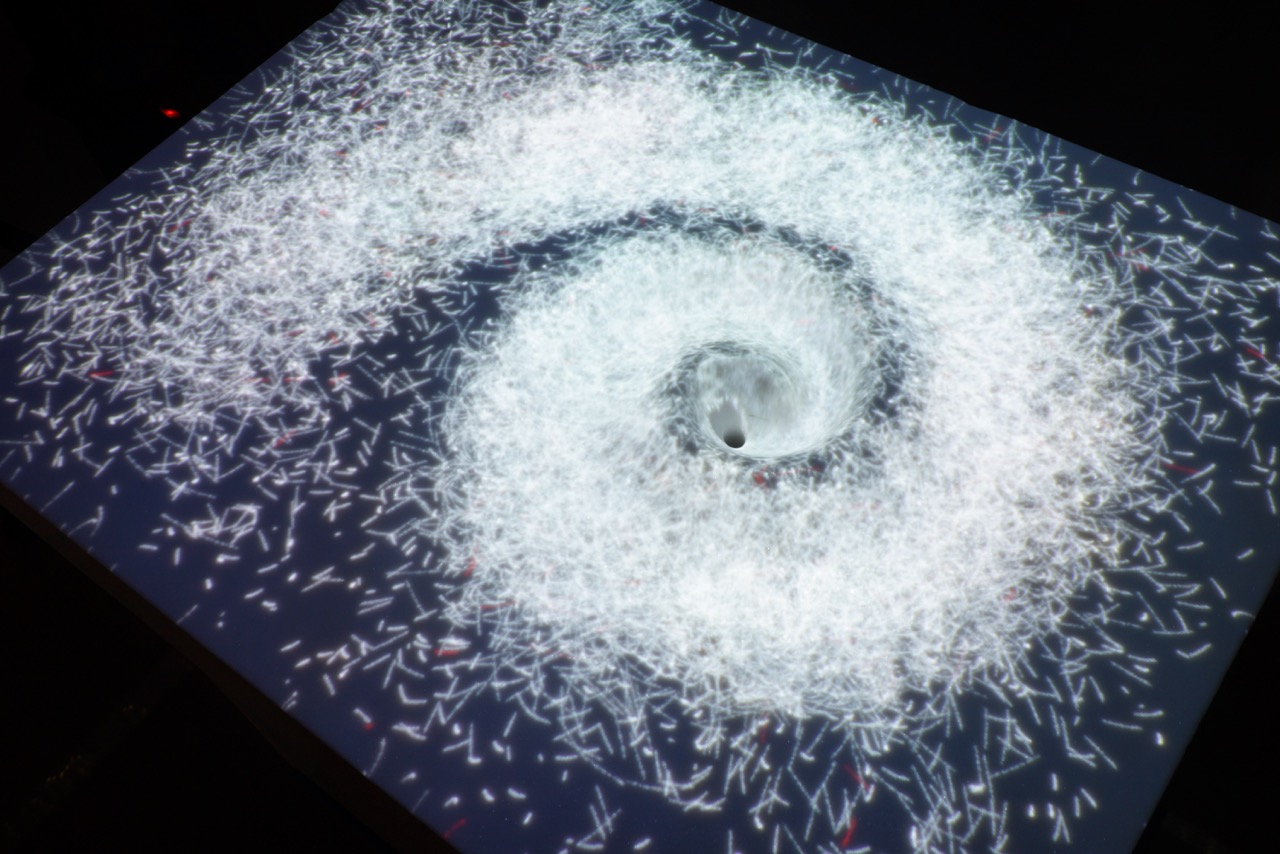
\includegraphics[width=0.7\textwidth]{galaksija}
        \end{center}
        \caption{Virtualno obogatena skulptura \cite{vodnjak}. Rezultate računalniško generirane animacije z video projektorjem projeciramo na kamnito skulpturo, da ustvarimo vtis, kot da bi po skulpturi polzele vodne kapljice \cite{video,solina2020skulpture}.}
        \label{pic1}
    \end{figure}


    \section{Podnapisi k slikam in tabelam}

    Vsaki sliki ali tabeli moramo dodati podnapis, ki na kratko pojasnjuje, kaj je na sliki ali tabeli.
    Če nekdo le prelista diplomsko delo, naj bi že iz slik in njihovih podnapisov lahko na grobo razbral, kakšno temo naloga obravnava.

    Če slike povzamemo iz drugih virov, potem se moramo v podnapisu k taki sliki sklicevati na ta vir!


    \chapter{Struktura strokovnih besedil}
    \label{stroka}

    Strokovna besedila imajo ustaljeno strukturo, da bi lahko hitreje in lažje brali in predvsem razumeli taka besedila, saj načeloma vemo vnaprej,
    kje v besedilu se naj bi nahajale določene informacije.

    Najbolj osnovna struktura strokovnega besedila je:
    \begin{description}
        \item[naslov besedila,] ki naj bo sicer kratek, a kljub temu dovolj poveden o vsebini besedila,
        \item[imena avtorjev] so običajno navedena po teži prispevka, prvi avtor je tisti, ki je besedilo dejansko pisal, zadnji pa tisti, ki je raziskavo vodil,
        \item[kontaktni podatki] -- poleg imena in naslova institucije je potreben vsaj naslov elektronske pošte,
        \item[povzetek] je kratko besedilo, ki povsem samostojno povzame vsebino in izpostavi predvsem glavne rezultate ali zaključke,
        \item[ključne besede] so tudi namenjene iskanju vsebin med množico člankov,
        \item[uvodno poglavje] uvede bralca v tematiko besedila, razloži kaj je namen besedila, predstavi področje o katerem besedilo piše
        (če temu ni namenjeno v celoti posebno poglavje) ter na kratko predstavi strukturo celotnega besedila,
        \item[poglavja] tvorijo zaokrožene celote, ki se po potrebi še nadalje členijo na podpoglavja, namenjena so recimo opisu orodij,
        ki smo jih uporabili pri delu, teoretičnim rezultatom ali predstavitvi rezultatov, ki smo jih dosegli,
        \item[zaključek] še enkrat izpostavi glavne rezultate ali ugotovitve, jih primerja z dosedanjimi in morebiti poda tudi ideje za nadaljno delo,
        \item[literatura] je seznam vseh virov, na katere smo se pri svojem delu opirali, oziroma smo se na njih sklicevali v svojem besedilu.
    \end{description}

    Naslove poglavij in podpoglavij izbiramo tako, da lahko bralec že pri prelistavanju diplome in branju naslovov
    v grobem ugotovi, kaj je vsebina diplomskega dela.

    Strokovna besedila običajno pišemo v prvi osebi množine, v nevtralnem in umirjenem tonu.
    Uporaba sopomenk ni zaželena, saj želimo zaradi lažjega razumevanja za iste pojme vseskozi uporabljati iste besede.
    Najpomembnejše ugotovitve je smiselno večkrat zapisati, na primer v povzetku, uvodu, glavnem delu in zaključku.
    Vse trditve naj bi temeljile bodisi na lastnih ugotovitvah (izpeljavah, preizkusih, testiranjih) ali pa z navajanjem ustreznih virov.

    Največ se lahko naučimo s skrbnim branjem dobrih zgledov takih besedil.


    \chapter{Pogoste napake pri pisanju v slovenščini}  % poglavje dodal Solina
    \label{slo}

    V slovenščini moramo paziti pri uporabi pridevnikov, ki se ne sklanjajo, kot so npr. kratice.
    Pravilno pišemo ``model CAD'' in \textbf{ne} ``CAD model''!

    Pri sklanjanju tujih imen ne uporabljamo vezajev, pravilno je Applov operacijski sistem in \textbf{ne} Apple-ov.

    Pika, klicaj in vprašaj so levostični: pred njimi ni presledka, za njimi pa je presledek.
    Klicajev in vprašajev se v strokovnih besedilih načeloma izogibamo. Oklepaji so desnostični in zaklepaji levostični: (takole).

    Z narekovaji označujemo premi govor, naslove, citate ali pa z njim dajemo besedam poseben pomen. Narekovaji so stična ločila. Ločimo različne narekovaje, vendar je v
    \LaTeX u najbolj enostavno uporabiti ``dvojni narekovaj zgoraj''. Za druge vrste narekovajev je potrebno uvoziti dodatne pakete ali fonte.
    Besede lahko vizualno označimo tudi z uporabo drugih pisav iz iste družine, npr.
    kurzivno in krepko pisavo, vendar pri uporabi teh fontov ne smemo pretiravati.

    Vezaj je levo in desno stičen, npr. \verb=slovensko-angleški slovar= in ga pišemo z enim znakom za pomišljaj.
    V slovenščini je presledek pred in po pomišljaju: Pozor -- hud pes! (\verb=Pozor -- hud pes!=).
    V angleščini pa je za razliko pomišljaj levo in desno stičen in se v \LaTeX u piše s tremi pomišljaji: \verb=---=.
    S stičnim pomišljajem pa lahko nadomeščamo predlog od \dots do, denimo pri navajanju strani, npr. preberite strani 7--11 (\verb=7--11=).

    ``Pred ki, ko, ker, da, če vejica skače''.
    To osnovnošolsko pravilo smo v življenju po potrebi uporabljali, dopolnili, morda celo pozabili.
    Pravilo sicer drži, ampak samo če je izpolnjenih kar nekaj pogojev (npr. da so ti vezniki samostojni, enobesedni, ne gre za vrivek itd.).
    Povedki so med seboj ločeni z vejicami, razen če so zvezani z in, pa, ter, ne–ne, niti–niti, ali, bodisi, oziroma.
    Sicer pa je bolje pisati kratke stavke kot pretirano dolge.

    V računalništvu se stalno pojavljajo novi pojmi in nove besede, za katere pogosto še ne obstajajo uveljavljeni slovenski izrazi.
    Kadar smo v dvomih, kateri slovenski izraz je primeren, si lahko pomagamo z iskanjem na kakšnem od slovenskih spletnih slovarjev~\cite{slovarji}, še posebej v
    \textit{Islovarju} Slovenskega društva Informatika \cite{Islovar} in Slovarju Slovenskega društva za razpoznavanje vzorcev~\cite{sdrv}.


    \chapter{Koristni nasveti pri pisanju v \LaTeX{u}}
    \label{latex}

    Programski paket \LaTeX\ je bil prvotno predstavljen v priročniku~\cite{lamport} in je v resnici nadgradnja sistema \TeX\ avtorja Donalda Knutha~\cite{knuth},
    znanega po svojih knjigah o umetnosti programiranja
    ter Knuth-Bendixovem algoritmu~\cite{knuth1983simple}.
    \TeX\ in njegove izpeljanke so odprtokodni programi.

    Različnih implementacij \LaTeX{}a je cela vrsta.
    Za OS X priporočamo TeXShop, za Windows PC pa MikTeX.
    Spletna verzija, ki poenostavi sodelovanje pri pisanju, je Overleaf.

    Včasih smo si pri pisanju v \LaTeX{}u pomagali predvsem s tiskanimi pri\-ro\-čni\-ki~\cite{lamport}, danes pa je enostavneje in hitreje, da ob vsakem problemu za pomoč enostavno povprašamo Google,
    saj je na spletu cela vrsta forumov za pomoč pri \TeX iranju.

    \LaTeX\ včasih ne zna pravilno deliti slovenskih besed, ki vsebujejo črke s streši\-ca\-mi.
    Če taka beseda štrli preko desnega roba,  lahko \LaTeX{}u pokažemo, kje se tako besedo deli takole: \verb=ra\-ču\-nal\-ni\-štvo=.
    Katere vrstice so predolge lahko vidimo tako, da dokument prevedemo s vključeno opcijo \texttt{draft}: \verb=\documentclass[a4paper, 12pt, draft]{book}=.

    Predlagamo, da v izvornem besedilu začenjate vsak stavek v novi vrstici, saj \LaTeX\ sam razporeja besede po vrsticah postavljenega besedila.
    Bo pa zato iskanje po izvornem besedilu in popravljanje veliko hitrejše.
    Večina sistemov za \TeX{}iranje sicer omogoča s klikanjem enostavno prestopanje iz prevedenega besedila na ustrezno mesto v izvornem besedilu in obratno.

    Boljšo preglednost dosežemo tako kot pri pisanju programske kode -- z vizualnim urejanjem kode in izpuščanjem praznih vrstic.
    Pri spreminjanju in dodajanju izvornega besedila je najbolje pogosto prevajati, da se sproti prepričamo, če so naši nameni pravilno izpolnjeni.

    Kadar besedilo, ki je že bilo napisano z nekim vizualnim urejevalnikom (npr. z Wordom), želimo prenesti v \LaTeX, je tudi najbolje to delati postopoma s posameznimi bloki besedila,
    tako da lahko morebitne napake hitro identificiramo in odpravimo.
    Za prevajanje Wordovih datotek v \LaTeX\ -- in obratno -- sicer obstajajo prevajalniki, ki pa običajno ne generirajo tako čisto logično strukturo besedila, kot jo sicer \LaTeX\ omogoča.
    Hiter in enostaven način prevedbe besedila, ki zahteva sicer ročne dopolnitve, lahko poteka tudi tako, da besedilo urejeno z vizualnim urejevalnikom najprej shranimo v formatu pdf,
    nato pa to besedilo uvozimo v urejevalnik, kjer urejamo izvorno besedilo v formatu \LaTeX.


    \section{Pisave v \LaTeX u}

    V  \LaTeX ovem okolju lahko načeloma uporabljamo poljubne pisave.
    Izbira poljubne pisave pa ni tako enostavna kot v vizualnih urejevalnikih besedil.
    Posamezne oblikovno medseboj usklajene pisave so običajno združene v družine pisav.
    V \LaTeX u se privzeta družina pisav imenuje Computer Modern,
    kjer so poleg navadnih črk (roman v \LaTeX u) na voljo tudi kurzivne črke (\textit{italic} v \LaTeX u),
    krepke (\textbf{bold} v \LaTeX u), kapitelke (\textsc{small caps} v \LaTeX u), linearne črke ({\textsf{san serif} v \LaTeX u}), pisava pisalnega stroja (\texttt{typewriter} v \LaTeX u) in nekatere njihove kombinacije, npr. krepke linearne črke
    ({\textbf{\textsf{san serif}} v \LaTeX u}).
    V istem dokumentu zaradi skladnega izleda uporabljamo običajno le pisave ene družine.
    Pomembna je tudi konsistentna raba večih pisav in da ne pretiravamo z mešanjem različnih pisav.

    Ko začenjamo uporabljati \LaTeX, je zato najbolj smiselno uporabljati kar privzete pisave, s katerimi je napisan tudi ta dokument.
    Z ustreznimi ukazi lahko nato preklapljamo med navadnimi, kurzivnimi, krepkimi in drugimi pisavami.
    Zelo enostavna je tudi izbira velikosti črk.
    \LaTeX\  odlično podpira večjezičnost, tudi v sklopu istega dokumenta, saj obstajajo pisave za praktično vse jezike, tudi take, ki ne uporabljajo latinskih črk.

    Za prikaz programske kode se pogosto uporablja pisava, kjer imajo vse črke enako širino, kot so črke na mehanskem pisalnem stroju ({\texttt{typewriter} v \LaTeX u}).

    Najbolj priročno okolje za pisanje kratkih izsekov programske kode je okolje \texttt{verbatim}, saj ta ohranja vizualno organizacijo izvornega besedila in ima privzeto pisavo pisalnega stroja.

    \begin{verbatim}
for (i = 0; i < 100; i++)
   for (j = i; j < 10; j++)
      some_function(i, j);
    \end{verbatim}


    \chapter{Kaj pa literatura?}
    \label{lit}

    Kot smo omenili že v uvodu, je pravi način za citiranje literature uporaba \BibLaTeX{a}~\cite{biblatex}.
    \BibLaTeX\ zagotovi, da pri določeni vrsti literature ne izpustimo
    nobene obvezne informacije
    in da vse informacije dosledno navajamo na enak način in po istem vrstnem redu.
    \BibLaTeX\ je nadgradnja starejšega sistema \BibTeX. Novejši sistem je bolje prilagojen slovenščini in navajanju spletnih virov. Sicer pa so starejše datoteke \texttt{.bib} kompatibilne z \BibLaTeX om.

    Osnovna ideja \BibLaTeX{a} je, da vse informacije o literaturi zapisujemo v posebno datoteko, v našem primeru je to \texttt{literatura.bib}.
    Vsakemu viru v tej datoteki določimo simbolično ime.
    V našem primeru je v tej datoteki nekaj najbolj značilnih zvrsti literature, kot so knjige~\cite{lamport},
    članki v revijah~\cite{leonardo} in zbornikih konferenc~\cite{ciuha2010visualization},
    poglavja v knjigah~\cite{poglavje_springer},
    spletni viri~\cite{slovarji,video},
    tehnično poročilo~\cite{andersen2012kinect},
    diplome~\cite{diploma} itd.
    Diploma~\cite{diploma} iz leta 1990 je bila prva diploma na tedanji Fakulteti za elektrotehniko in računalništvo, ki je bila oblikovana z \LaTeX om!
    Reference, ki so na spletnih straneh arhivirane v elektronski obliki, imajo običajno  \v stevilko DOI (\url{http://dx.doi.org}), ki jo tudi lahko vključimo v izpis literature in tako bralcu elektronske verzije naše publikacije ponudimo neposredno povezavo do elektronske kopije te reference.

    Po vsaki spremembi pri sklicu na literaturo moramo najprej prevesti izvorno besedilo s prevajalnikom \LaTeX, nato s prevajalnikom  \BibLaTeX, ki ustvari datoteko  {\tt vzorec\_dip\_Seminar.bbl}, in nato še dvakrat s prevajalnikom  \LaTeX.
    V okolju Overleaf je to večkratno prevajanje z različnimi prevajalniki uporabniku skrito. Zato tudi začetnim uporabnikom \LaTeX a svetujemo uporabo Overleafa.

    Kako se spisek literature nato izpiše (ali so posamezni viri razvrščeni po vrstnem redu sklicevanja, ali po abecedi priimkov prvih avtorjev, ali se imena avtorjev pišejo pred priimki itd.) je odvisno od parametrov paketa \BibLaTeX.
    V diplomi bomo uporabili parametre
    \texttt{style=numeric}, kar pomeni, da bodo sklici na literaturo v besedilu označeni z zaporednimi številkami, za vrstni red izpisa referenc pa
    \texttt{sorting=nty}, kar pomeni, da bodo reference urejene po priimkih prvih avtorjev, nato po naslovu reference in nazadnje po letu izdaje~\cite{ctan}.
    Zato je potrebno pri določenih zvrsteh literature, ki nima avtorjev, dodati parameter \texttt{key}, ki določi vrstni red vira po abecedi.

    Ko začenjamo uporabljati \BibLaTeX\ je lažje, če za urejanje datoteke \texttt{.bib} uporabljamo kar isti urejevalnik kot za urejanje datotek \texttt{.tex},
    čeprav obstajajo tudi posebni urejevalniki oziroma programi za delo z datotekami \texttt{.bib}.

    Le če se na določen vir v besedilu tudi sklicujemo, se bo ta vir pojavil tudi v spisku literature.
    Tako je avtomatično zagotovljeno, da se na vsak vir v seznamu literature tudi sklicujemo v besedilu diplome.
    V datoteki \texttt{.bib} imamo sicer lahko veliko več virov za literaturo, kot jih bomo uporabili v diplomi.


    \section{Zbiranje virov za seznam literature}

    Vire v formatu \texttt{.bib}  lahko enostavno poiščemo in prekopiramo iz spletnih strani založnikov ali različnih akademskih spletnih portalov za iskanje znanstvene literature.
    Izvoz referenc v Google učenjaku še dodatno poenostavimo, če v nastavitvah izberemo \BibTeX\ kot želeni format za izvoz navedb.
    Navedbe, ki jih prekopiramo iz Google učenjaka in drugih podobnih akademskih portalov, moramo pred uporabo nujno preveriti, saj so taki navedki pogosto generirani povsem avtomatično in lahko vsebujejo napačne ali nepopolne podatke.
    Najpogosteje je napačen tip publikacije!

    Pri sklicevanju na literaturo na koncu stavka moramo paziti, da je pika po ukazu \verb=\cite{ }=.
    Da \LaTeX\ ne bi delil vrstico ravno tako, da bi sklic na literaturo v oglatih oklepajih začel novo vrstico, lahko pred sklicem na literaturo dodamo nedeljiv presledek: \verb=~\cite{ }=.

    Običajno se v besedilu sklicujemo na nek vir ali več virov na koncu trdilnega stavka.
    Kadar pa omenimo avtorja nekega vira, pa sklic običajno vstavimo za njegovim priimkom.


    Dandanes se skoraj vsi pri iskanju informacij vedno najprej lotimo iskanja preko svetovnega spleta.
    Rezultati takega iskanja pa so pogosto spletne strani, ki danes obstajajo, jutri pa jih morda ne bo več, ali pa vsaj ne v taki obliki, kot smo jo prebrali.
    Smisel navajanja literature pa je, da tudi po dolgih letih nekdo, ki bo bral vašo diplomo, lahko poišče vire, ki jih navajate v diplomi.

    Znanstveni rezultati, ki so objavljeni v obliki recenziranih člankov, bodisi v konferenčnih zbornikih, še bolje pa v znanstvenih revijah, so veliko bolj izčiščen in zanesljiv vir informacij, saj
    so taki članki šli skozi recenzijske postopke. Predvsem pa so taki članki stabilen vir informacij, saj se načeloma po njihovi objavi ne spreminjajo več.
    Skoraj vsi ti članki so dandanes dosegljivi tudi v elektronski obliki, bodisi v arhivih založnikov, univerzitetnih repozitorijih ali tudi na osebnih spletnih straneh njihovih avtorjev.
    Zato na svetovnem spletu začenjamo iskati vire za strokovna besedila predvsem preko akademskih spletnih portalov, kot so npr. Google učenjak, Research Gate ali Academia, saj so na teh portalih rezultati iskanja le akademske publikacije.
    Če je za dostop do nekega članka potrebno plačati, se obrnemo za pomoč in dodatne informacije na našo knjižnico.

    Za označevanje člankov, ki so na voljo v elektronski obliki, se je v zadnjem času uveljavila oznaka DOI
    (\url{https://www.doi.org}), kar močno olajša iskanje teh referenc na spletu.
    Založniki tudi starejšim člankom, ki so na voljo v elektronski obliki, za nazaj določajo oznake DOI.
    Zato poskusite poiskati ustrezno oznako DOI za vsak članek, ki ga citirate in jo vključite v seznam literature.

    Če res ne gre drugače, pa je pomembno, da pri sklicevanju na običajni spletni vir vedno navedemo tudi datum, kdaj smo dostopali do tega vira.

    Z uporabo \BibLaTeX{a} je možno natisniti seznam literature posebej za določene vrste referenc, na primer za članke v znanstvenih revijah, članke v konferenčnih zbornikih in poglavja v knjigah, kot je prikazano tudi v tem vzorcu diplome. Pri zbiranju literature si zato prizadevajte čimbolj napolniti sezname teh treh vrst referenc.


    \chapter{Skladnost s standardom PDF/A}
    \label{PDF}


    Elektronsko verzijo diplome je potrebno oddati preko sistema STUDIS v formatu PDF/A ~\cite{howtopdfa,pdfa},
    natančneje v formatu PDF/A-1b.
    PDF/A format je namenjen dolgoročnemu arhiviranju elektronskih dokumentov.
    Dokument v formatu PDF/A mora vsebovati vse potrebne informacije za prikazovanje in tiskanje dokumenta. To pomeni, da mora dokument vsebovati vso besedilo, vse slike, fonte in barvne informacije.
    Prva verzija standarda PDF/A, to je PDF/A-1 je bil objavljena leta 2005.
    Standard PDF/A-1 določa dva nivoja skladnosti: PDF/A-1a in PDF/A-1b.
    Nivo a (accesible) mora ustrezati vsem zahtevam standarda.
    Nivo b (basic) pa zahteva le, da se ohrani vizualni izgled dokumenta.
    Diplome, ki jih je potrebno oddati na sistemu STUDIS, morajo ustrezati nivoju standarda
    PDF/A-1b.

    \LaTeX\ in omenjeni format imata še nekaj težav s sobivanjem.
    Paket \texttt{pdfx.sty}, ki naj bi \LaTeX{u} omogočal podporo formatu PDF/A ne deluje vedno
    v skladu s pričakovanji.

    Zato raje priporočamo uporabo enega od mnogih spletnih mest, ki omo\-go\-ča\-jo konverzijo pdf datotek v obliko,
    ki je skladna s standardom PDF/A-1b, npr. \url{https://pdf.online/pdf-to-pdfa}, kjer je
    možno tudi testirati, ali je neka pdf datoteka skladna s tem standardom.

    V predlogi so poleg izvornega dokumenta \texttt{diploma-FRI-vzorec.tex}, še vložena slika \texttt{galaksija.jpeg}, datoteka \texttt{literatura.bib} za uporabljeno literaturo ter
    ikone za licenco Creative Commons.


    \chapter{Sklepne ugotovitve}

    Uporaba \LaTeX{a} in \BibLaTeX{a} je v okviru Diplomskega seminarja \textbf{obvezna}!
    Izbira -- \LaTeX\ ali ne \LaTeX\ -- pri pisanju dejanske diplomske naloge pa je pre\-pu\-šče\-na dogovoru med diplomantom in njegovim mentorjem.

    Res je, da so prvi koraki v \LaTeX{}u težavni.
    Ta dokument naj služi kot začetna opora pri hoji.
    Pri kakršnihkoli nadaljnih vprašanjih ali napakah pa svetujemo uporabo Googla, saj je spletnih strani za pomoč pri odpravljanju težav pri uporabi \LaTeX{}a ogromno.

    Preden diplomo oddate na sistemu STUDIS, še enkrat preverite, če so slovenske besede, ki vsebujejo črke s strešicami,  pravilno deljene in da ne segajo preko desnega roba.
    Poravnavo po vrsticah lahko kontrolirate tako, da izvorno datoteko enkrat testno prevedete z opcijo \texttt{draft}, kar vam pokaže predolge vrstice.


%\cleardoublepage
%\addcontentsline{toc}{chapter}{Literatura}

    \printbibliography[heading=bibintoc,type=article,title={Članki v revijah}]

    \printbibliography[heading=bibintoc,type=inproceedings,title={Članki v zbornikih}]

    \printbibliography[heading=bibintoc,type=incollection,title={Poglavja v knjigah}]

    \printbibliography[heading=bibintoc,title={Celotna literatura}]


\end{document}

